\documentclass[11pt]{article}

\usepackage[margin=1in]{geometry}
\usepackage{amsmath, amssymb, amsfonts, amsthm}
\usepackage{amscd}
\usepackage{enumitem}
\usepackage[colorlinks=true, linkcolor=blue, urlcolor=blue]{hyperref}
\usepackage{tikz}
\usetikzlibrary{arrows.meta,calc}
\colorlet{ref}{black!40}      % reference object (before)
\colorlet{img}{blue!62}       % image / deformed object (after)
% one uniform thumbnail cell: #1 = tikz body, #2 = name, #3 = invariant tag
\newcommand{\gicon}[3]{%
  \begin{minipage}[t]{0.232\linewidth}\centering
    \begin{tikzpicture}[scale=0.5,line join=round,line cap=round,>={Stealth[length=4pt]}]#1\end{tikzpicture}\\[1pt]
    {\scriptsize\textbf{#2}}\\{\scriptsize\itshape #3}\par\vspace{3pt}
  \end{minipage}}

\theoremstyle{definition}
\newtheorem{definition}{Definition}[section]
\newtheorem{example}{Example}[section]
\theoremstyle{remark}
\newtheorem{remark}{Remark}[section]
\newtheorem*{keyidea}{Key idea}
\newtheorem*{verdict}{Verdict}

\newcommand{\g}{\mathfrak{g}}
\newcommand{\R}{\mathbb{R}}
\newcommand{\pd}[2]{\frac{\partial #1}{\partial #2}}
\newcommand{\Spec}{\operatorname{Spec}}
\newcommand{\Sol}{\operatorname{Sol}}
\newcommand{\Vect}{\operatorname{Vect}}
\newcommand{\sltwo}{\mathfrak{sl}_2}

\title{\bf From Lie Symmetry to Machine Learning:\\
a conceptual map for semi-analytical PDE solving}
\author{LieML project --- scoping note}
\date{\today}

\begin{document}
\maketitle

\begin{abstract}
This note is a self-contained, beginner-friendly map of the ideas behind the project
\emph{``Semi-Analytical and Machine-Learning Methods for Solving PDEs Using Lie Symmetry Analysis.''}
It assumes little prior exposure to Lie groups or to how the symmetries of a partial differential
equation (PDE) are classified. It builds the picture in three layers --- continuous symmetry,
symmetry \emph{reduction} (your ``variable compression'' intuition, made precise), and the
PDE\,--\,Lie\,--\,ML triangle --- and then answers two questions directly: (i) \emph{should you study
finite groups of Lie type and their topology?} and (ii) \emph{is a ``combinatorial method'' useful for
analysing PDE--Lie, ML--Lie, and PDE--ML correlations?} Throughout, the abstract claims are anchored to
small computations that have already been run and verified for this project (Burgers, the heat equation,
the porous-medium equation, and Fisher--KPP).
\end{abstract}

\tableofcontents

\section{The one-sentence picture}

A PDE is hard for two reasons: it has \emph{many independent variables} and an \emph{enormous solution
space}. A continuous symmetry is a knob you can turn that sends solutions to solutions. The central fact
of the subject is:

\begin{keyidea}
Each independent ``symmetry knob'' lets you \emph{remove one independent variable} from the problem.
Turning the knobs in the right order \emph{compresses} a PDE in several variables down to an ordinary
differential equation (ODE) in one variable --- which you can often solve exactly or with a short series.
\end{keyidea}

So your instinct is exactly right: \textbf{Lie theory is a ``variable-compression'' tool.} The rest of
this note explains \emph{why} that works, \emph{how} the symmetries are found and classified, and where
machine learning (ML) fits in.

\medskip
\noindent\emph{A familiar special case you already know.} Dimensional analysis (the Buckingham
$\Pi$-theorem) is precisely symmetry reduction for the \emph{scaling} symmetry: it replaces several
dimensional variables by fewer dimensionless groups. Lie theory is the systematic generalisation to
\emph{all} continuous symmetries, not just scalings.

\section{Lie groups and Lie algebras, gently}

\subsection{Continuous symmetry: one-parameter groups}

\begin{definition}[One-parameter group of transformations]
A family of maps $g_\varepsilon$ depending smoothly on a real parameter $\varepsilon$ with
$g_0=\mathrm{id}$ and $g_{\varepsilon_1}\circ g_{\varepsilon_2}=g_{\varepsilon_1+\varepsilon_2}$.
\end{definition}

Examples on the plane $(x,t)$ or on $(x,t,u)$:
\begin{itemize}[nosep]
  \item \textbf{Translation:} $g_\varepsilon:(x)\mapsto(x+\varepsilon)$.
  \item \textbf{Scaling:} $g_\varepsilon:(x)\mapsto(e^{\varepsilon}x)$.
  \item \textbf{Rotation:} $g_\varepsilon:(x,t)\mapsto(x\cos\varepsilon-t\sin\varepsilon,\;x\sin\varepsilon+t\cos\varepsilon)$.
\end{itemize}

A \textbf{Lie group} is, informally, a group that is simultaneously a smooth surface (a manifold), so
that ``move a little'' makes sense. The examples above are the building blocks $(\R,+)$,
$(\R_{>0},\times)$, and $SO(2)$.

\subsection{The infinitesimal generator: linearise the knob}

The decisive simplification is to look at a transformation \emph{near $\varepsilon=0$}. Differentiating
the orbit gives a velocity field --- a \textbf{vector field} --- called the \emph{infinitesimal
generator}:
\[
X \;=\; \xi(x,t,u)\,\pd{}{x} + \tau(x,t,u)\,\pd{}{t} + \phi(x,t,u)\,\pd{}{u},
\qquad
(\xi,\tau,\phi)=\left.\frac{d}{d\varepsilon}\right|_{\varepsilon=0} g_\varepsilon .
\]
The set of all such generators, equipped with the commutator bracket
$[X,Y]=XY-YX$, is the \textbf{Lie algebra} $\g$ of the group.

\begin{keyidea}[Why the algebra is the workhorse]
The group law is \emph{nonlinear}, but the generators form a \emph{linear} space. Lie's theorems say the
whole local group is recovered from its generators by the exponential (the flow of the vector field),
\[
g_\varepsilon=\exp(\varepsilon X).
\]
So we trade a hard nonlinear search over groups for a \emph{linear} computation over generators. This
is exactly why symmetry analysis is \emph{algorithmic}.
\end{keyidea}

\begin{remark}[``Finite-dimensional'' means the \emph{algebra}, not a finite group]
When people say a PDE has a ``finite-dimensional symmetry algebra'' they mean $\g$ is a finite-dimensional
\emph{vector space} (e.g.\ dimension $5$ for Burgers below). This has nothing to do with \emph{finite
groups}. We return to this important point in \S\ref{sec:finite}.
\end{remark}

\subsection{What a manifold is --- and what makes a group a Lie group}
\label{sec:manifold}

We have been saying ``a Lie group is a group that is also a smooth manifold.'' That one sentence carries
the whole subject, so we now unpack it word by word, starting from nothing more than the idea of a
continuous map. Everything in \S2.1--2.2 --- ``move a little'', the velocity field $X$, the exponential ---
is legitimate \emph{only because} the underlying object is a smooth manifold, a space on which calculus
makes sense. (For the topology in full, the standard gentle reference is Lee,
\emph{Introduction to Smooth Manifolds}; the \texttt{lee\_smooth\_manifolds} PDF in \texttt{ref/}.)

\paragraph{Step 1 --- continuity and homeomorphism.}
\begin{definition}[Topological space; homeomorphism]
A \textbf{topological space} is a set together with a chosen collection of ``open'' subsets --- a
declaration of which points count as \emph{near} each other --- just enough structure to say when a map is
\textbf{continuous} (preimages of open sets are open). A \textbf{homeomorphism} is a continuous bijection
$f:X\to Y$ whose inverse $f^{-1}$ is also continuous. When one exists, $X$ and $Y$ are
\textbf{homeomorphic}: ``the same up to continuous deformation,'' with no cutting and no gluing.
\end{definition}

\begin{example}[Topologically the same, or not]
The open interval $(-1,1)$ is homeomorphic to the whole line $\R$ (e.g.\ via $x\mapsto\tan(\pi x/2)$); the
proverbial coffee mug is homeomorphic to a doughnut. But a circle is \emph{not} homeomorphic to a line
segment --- you would have to cut it. Homeomorphism is the right notion of ``same shape'' \emph{before} any
distance or smoothness is imposed.
\end{example}

\paragraph{Step 2 --- locally Euclidean.}
\begin{definition}[Locally Euclidean]
A space $M$ is \textbf{locally Euclidean of dimension $n$} if every point $p\in M$ has an open neighbourhood
$U$ that is homeomorphic to an open subset of $\R^n$. In words: \emph{up close, $M$ looks like flat
$\R^n$.}
\end{definition}
This is the Earth-looks-flat-locally idea made exact: the globe is curved, yet any city fits on a flat
street map. For a connected space the number $n$ is the same at every point; it is the \textbf{dimension}
of $M$.

\paragraph{Step 3 --- charts and atlases.}
\begin{definition}[Chart, atlas, transition map]
A \textbf{chart} is a homeomorphism $\varphi:U\to\varphi(U)\subseteq\R^n$ from an open set $U\subseteq M$;
it is a local \emph{coordinate system}, attaching numbers $(x^1,\dots,x^n)$ to the points of $U$. An
\textbf{atlas} is a family of charts whose domains cover $M$. Where two charts overlap, the
\textbf{transition map} $\varphi_\beta\circ\varphi_\alpha^{-1}$ re-expresses one set of coordinates in
terms of the other (Fig.~\ref{fig:chart}).
\end{definition}

\begin{figure}[h]
\centering
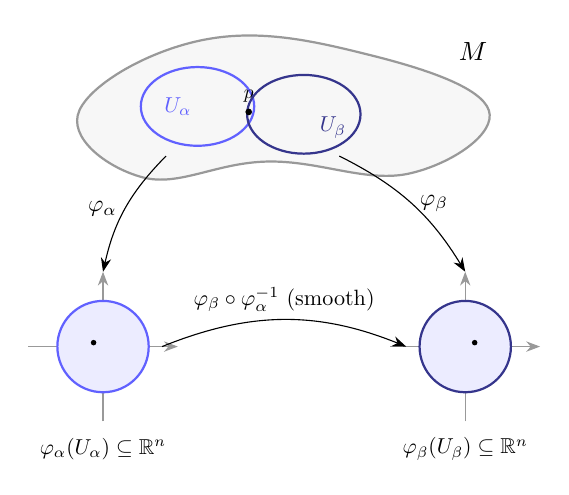
\begin{tikzpicture}[>={Stealth[length=5pt]},line join=round,scale=1.0]
  % --- the manifold M (top) ---
  \draw[ref,thick,fill=ref!8] plot[smooth cycle,tension=0.7]
     coordinates {(-2.6,2.0)(-1.0,2.9)(1.1,2.7)(2.6,2.0)(1.6,1.2)(-0.2,1.35)(-1.8,1.15)};
  \node[scale=0.95] at (2.4,2.75) {$M$};
  \draw[img,thick] (-1.1,2.05) ellipse (0.72 and 0.5);
  \node[img,scale=0.78] at (-1.35,2.05) {$U_\alpha$};
  \draw[img!55!black,thick] (0.25,1.95) ellipse (0.72 and 0.5);
  \node[img!55!black,scale=0.78] at (0.62,1.78) {$U_\beta$};
  \fill[black] (-0.45,1.98) circle (1.2pt) node[above=1pt,scale=0.7]{$p$};
  % --- chart maps ---
  \draw[->] (-1.5,1.42) to[bend right=16] node[left,scale=0.85]{$\varphi_\alpha$} (-2.3,-0.05);
  \draw[->] (0.7,1.42) to[bend left=16] node[right,scale=0.85]{$\varphi_\beta$} (2.3,-0.05);
  % --- left coordinate region ---
  \begin{scope}[shift={(-2.3,-1.0)}]
    \draw[ref,thin,->] (-0.95,0)--(0.95,0); \draw[ref,thin,->] (0,-0.95)--(0,0.95);
    \fill[img!12] (0,0) circle (0.58); \draw[img,thick] (0,0) circle (0.58);
    \fill[black] (-0.12,0.05) circle (1.0pt);
    \node[scale=0.78] at (0,-1.3) {$\varphi_\alpha(U_\alpha)\subseteq\R^n$};
  \end{scope}
  % --- right coordinate region ---
  \begin{scope}[shift={(2.3,-1.0)}]
    \draw[ref,thin,->] (-0.95,0)--(0.95,0); \draw[ref,thin,->] (0,-0.95)--(0,0.95);
    \fill[img!12] (0,0) circle (0.58); \draw[img!55!black,thick] (0,0) circle (0.58);
    \fill[black] (0.12,0.05) circle (1.0pt);
    \node[scale=0.78] at (0,-1.3) {$\varphi_\beta(U_\beta)\subseteq\R^n$};
  \end{scope}
  % --- transition map ---
  \draw[->] (-1.55,-1.0) to[bend left=22]
     node[above,scale=0.8]{$\varphi_\beta\circ\varphi_\alpha^{-1}$ (smooth)} (1.55,-1.0);
\end{tikzpicture}
\caption{\textbf{A manifold and its charts.} Each point of the curved space $M$ has a neighbourhood
($U_\alpha$, $U_\beta$) carried by a chart ($\varphi_\alpha$, $\varphi_\beta$) onto a flat patch of
$\R^n$ --- this is what \emph{locally Euclidean} means. On the overlap (containing $p$) the two coordinate
systems are related by the \emph{transition map} $\varphi_\beta\circ\varphi_\alpha^{-1}$; requiring every
such transition to be infinitely differentiable is exactly what makes $M$ a \emph{smooth} manifold.}
\label{fig:chart}
\end{figure}

\paragraph{Step 4 --- topological and smooth manifolds.}
\begin{definition}[Manifold]
A \textbf{topological manifold} of dimension $n$ is a space that is (i) \emph{locally Euclidean} of
dimension $n$, (ii) \emph{Hausdorff} (any two points lie in disjoint open sets --- no ``doubled'' points),
and (iii) \emph{second-countable} (its topology has a countable base --- it is not pathologically large).
It is a \textbf{smooth ($C^\infty$) manifold} if it carries an atlas whose transition maps are all
infinitely differentiable.
\end{definition}

\begin{keyidea}[Why ``smooth'' is the whole point]
Smooth transition maps are exactly what let calculus pass from one chart to another \emph{unambiguously}:
whether a function is differentiable, and what its derivative is, cannot depend on which coordinate system
you happened to pick. On a smooth manifold one can therefore define smooth functions, differentiate them,
and --- decisively for us --- define \emph{tangent vectors} and \emph{vector fields} without ever leaving
the abstract space. The generator $X$ of \S2.2 lives here.
\end{keyidea}

\begin{definition}[Tangent space]
The \textbf{tangent space} $T_pM$ at a point $p$ is the $n$-dimensional vector space of velocities
$\dot\gamma(0)$ of smooth curves $\gamma$ passing through $p$. A \textbf{vector field} chooses one tangent
vector $X_p\in T_pM$ at every point, smoothly --- precisely the
$\xi\,\partial_x+\tau\,\partial_t+\phi\,\partial_u$ of \S2.2.
\end{definition}

\paragraph{Step 5 --- a Lie group.}
\begin{definition}[Lie group]
A \textbf{Lie group} is a set $G$ that is \emph{simultaneously}
\begin{itemize}[nosep]
  \item a \textbf{group} --- an associative product with an identity $e$ and inverses --- and
  \item a \textbf{smooth manifold},
\end{itemize}
with the two structures \emph{compatible}: multiplication $G\times G\to G,\ (g,h)\mapsto gh$ and inversion
$G\to G,\ g\mapsto g^{-1}$ are \emph{smooth} maps. Its \textbf{dimension} is its dimension as a manifold ---
the number of independent continuous parameters (the ``knobs'' of \S2.1).
\end{definition}

\begin{keyidea}[Where the Lie algebra comes from]
Because $G$ is a smooth manifold, it has a tangent space at the identity, and \emph{that} is the Lie
algebra: $\g:=T_eG$. The infinitesimal generators of \S2.2 are exactly the elements of $T_eG$, and the
bracket $[X,Y]$ measures how the group multiplication fails to commute near $e$. Smoothness of the group
operations is what makes the exponential $\exp:\g\to G$ a local diffeomorphism --- the rigorous form of
``recover the local group from its generators'' (\S2.2). In particular $\dim G=\dim\g$: the circle is
$1$-dimensional, $SO(3)$ is $3$-dimensional, $GL(n,\R)$ is $n^2$-dimensional.
\end{keyidea}

\begin{example}[The circle: the cleanest Lie group]
The unit circle $SO(2)=\{e^{i\theta}\}$ is a $1$-dimensional smooth manifold (one angle coordinate), and
angle addition $e^{i\theta}e^{i\phi}=e^{i(\theta+\phi)}$ is smooth --- so it is a Lie group. It already
illustrates why charts are unavoidable: \emph{no single} chart covers the whole circle (any angle
coordinate must jump somewhere), so the smallest atlas needs two overlapping arcs. Locally the circle is
just $\R$; globally it closes up --- it is \emph{compact}.
\end{example}

\begin{remark}[Manifold $\ne$ Lie group]
Every Lie group is a manifold, but most manifolds are \emph{not} Lie groups. The $2$-sphere $S^2$ carries
no continuous group law at all (relatedly, you cannot comb a smooth nonvanishing vector field on it --- the
``hairy ball'' theorem); among spheres only $S^1=U(1)$ and $S^3=SU(2)$ are Lie groups. The group structure
is a genuine extra constraint on top of being a smooth space.
\end{remark}

\paragraph{Step 6 --- back to matrices.}
This abstract picture is realised concretely by the \textbf{matrix Lie groups} of the next subsection,
which are the hands-on manifolds to keep in mind:
\begin{itemize}[nosep]
  \item $GL(n,\R)$ is an \emph{open} subset of the $n^2$-dimensional space of all real matrices (the
        condition $\det\neq0$ is open), hence a manifold of dimension $n^2$ described by a single global
        chart.
  \item $O(n)$, $SO(n)$, $U(n)$, $\dots$ are \emph{level sets} cut out by smooth equations such as
        $A^{\top}A=I$: curved ``surfaces'' sitting inside matrix space, i.e.\ embedded submanifolds.
\end{itemize}
\begin{keyidea}[Closed-subgroup theorem: why ``closed'' buys smoothness]
Cartan's \textbf{closed-subgroup theorem} states that \emph{any} subgroup of $GL(n,\mathbb{C})$ that is
topologically closed is automatically a smooth embedded submanifold --- hence a Lie group. This is exactly
why the matrix definition of \S\ref{sec:matrix} needs only the single word \emph{closed}: smoothness, the
tangent space, and the exponential all come for free. Matrix Lie groups are therefore the most concrete
manifolds to picture --- surfaces in matrix space on which $\exp$, the bracket, and representations become
ordinary linear algebra.
\end{keyidea}

\subsection{A concrete model to hold onto: matrix (linear) Lie groups}
\label{sec:matrix}

The manifold definition above is correct but abstract. The fastest rigorous on-ramp --- and the viewpoint
of B.~C.~Hall, \emph{Lie Groups, Lie Algebras, and Representations: An Elementary Introduction} --- is to
make everything \emph{matrices}.

\begin{definition}[Matrix (linear) Lie group]
A \textbf{matrix Lie group} is a closed subgroup of the general linear group $GL(n,\mathbb{C})$
(invertible $n\times n$ complex matrices). Examples: $SL(n)$ (determinant $1$), $O(n)$ and $SO(n)$
(orthogonal / rotations), $U(n)$ and $SU(n)$ (unitary), and the Heisenberg and Euclidean groups.
\end{definition}

In this model the three abstract notions of \S2.1--2.2 become elementary linear algebra:
\begin{itemize}[nosep]
  \item \textbf{Group $\to$ algebra via the matrix exponential.} $\exp(A)=\sum_{k\ge0}A^k/k!$, and a
        one-parameter subgroup is $g(t)=\exp(tX)$ --- the matrix analogue of $g_\varepsilon=\exp(\varepsilon X)$.
  \item \textbf{The Lie algebra is a space of matrices.} $\g=\{\,X:\exp(tX)\in G\ \text{for all }t\in\R\,\}$,
        a real vector space closed under the \emph{commutator} $[X,Y]=XY-YX$. Concretely
        $\mathfrak{so}(n)$ = skew-symmetric matrices, $\mathfrak{sl}(n)$ = traceless matrices,
        $\mathfrak{su}(n)$ = skew-Hermitian \emph{and} traceless matrices (skew-Hermitian alone is $\mathfrak{u}(n)$).
        Note $O(n)$ and $SO(n)$ share the \emph{same} algebra $\mathfrak{so}(n)$ --- the algebra only sees the identity component.
  \item \textbf{The bracket measures non-commutativity (Baker--Campbell--Hausdorff).}
        $\exp(X)\exp(Y)=\exp\!\big(X+Y+\tfrac12[X,Y]+\cdots\big)$, so the single bracket already controls
        how the group fails to commute --- the precise sense in which ``the algebra knows the local group.''
\end{itemize}

\begin{keyidea}[Representations --- the bridge to ML]
A \textbf{representation} is a homomorphism $\rho:G\to GL(V)$ (or $\g\to\mathfrak{gl}(V)$): it records
\emph{how the group acts linearly} on a vector space $V$. PDE solution spaces and ML feature spaces are
exactly such $V$'s. Then ``symmetry of a PDE'' and ``equivariance of a network'' become the \emph{same}
statement --- a map that intertwines two representations,
$\rho_{\text{out}}(g)\,\Phi=\Phi\circ\rho_{\text{in}}(g)$. Representation theory (the third pillar of
Hall's book) is the common language of the PDE--Lie--ML triangle (\S\ref{sec:triangle}).
\end{keyidea}

\begin{remark}[How the matrix picture connects to the vector-field picture]
For PDE symmetry the group acts on $(x,t,u)$-space and the generators are \emph{vector fields} (\S2.2),
whose action can be \emph{nonlinear}. Matrix Lie groups are the cleanest \emph{linear} special case --- the
right place to first meet $\exp$, the bracket, BCH and representations --- and prolongation (letting $X$ act
on derivatives) is itself representation-theoretic: the group acts linearly on the ``jet'' of derivatives.
Linear actions also dominate the ML side (equivariant layers), so Hall's matrix route is the most efficient
bridge for this project.
\end{remark}

\subsection{A catalogue of the classical groups (and their special/unitary cases)}
\label{sec:catalogue}

The matrix groups of \S\ref{sec:matrix} fall into a few families, each defined by the \emph{structure it
preserves}: a volume, a real inner product, a Hermitian form, or a symplectic form. Two prefixes recur.
\textbf{Special} ($S$) means \emph{determinant $1$} (volume/orientation preserving); \textbf{unitary}
($U$) means \emph{preserves a Hermitian form} (the complex analogue of orthogonal). Every symmetry
algebra met in PDE analysis is a subalgebra of one of these, or of an \emph{inhomogeneous} (translation)
extension of one (Table~B). Each group below is also drawn as an icon in Fig.~\ref{fig:zoo}.

\medskip
\noindent\textbf{Table A. The classical (linear) Lie groups.}
\begin{center}
\small
\setlength{\tabcolsep}{4.5pt}
\renewcommand{\arraystretch}{1.15}
\begin{tabular}{l l c c}
\hline
\textbf{Group} & \textbf{Preserves / defining condition} & $\dim_{\mathbb R}$ & \textbf{Compact} \\ \hline
$GL(n,\R)$ & invertible real matrices ($\det\neq0$) & $n^2$ & no \\
$SL(n,\R)$ & \quad$+$ volume: $\det=1$ & $n^2-1$ & no \\
$GL(n,\mathbb{C})$ & invertible complex matrices & $2n^2$ & no \\
$SL(n,\mathbb{C})$ & \quad$+\ \det=1$ & $2(n^2-1)$ & no \\ \hline
$O(n)$ & real symmetric form: $A^{\top}A=I$ (lengths) & $\tfrac12 n(n-1)$ & yes \\
$SO(n)$ & \quad$+\ \det=1$ (rotations) & $\tfrac12 n(n-1)$ & yes \\
$O(p,q)$ & real form of signature $(p,q)$ & $\tfrac12 (p{+}q)(p{+}q{-}1)$ & no \\
$SO^{+}(1,3)$ & \textbf{Lorentz}, proper orthochronous & $6$ & no \\
$O(n,\mathbb{C}),\,SO(n,\mathbb{C})$ & complex orthogonal & $n(n-1)$ & no \\ \hline
$U(n)$ & Hermitian form: $A^{*}A=I$ & $n^2$ & yes \\
$SU(n)$ & \quad$+\ \det=1$ & $n^2-1$ & yes \\
$U(p,q)$ & Hermitian form of signature $(p,q)$ & $(p{+}q)^2$ & no \\
$SU(p,q)$ & \quad$+\ \det=1$ & $(p{+}q)^2-1$ & no \\ \hline
$Sp(2n,\R)$ & real symplectic (antisymmetric) form & $n(2n{+}1)$ & no \\
$Sp(n)=USp(2n)$ & compact symplectic $=Sp(2n,\mathbb{C})\cap U(2n)$ & $n(2n{+}1)$ & yes \\
$Sp(2n,\mathbb{C})$ & complex symplectic & $2n(2n{+}1)$ & no \\ \hline
\end{tabular}
\end{center}
\noindent{\small\emph{Coincidences:} $SO(2)=U(1)$ (the circle); $Sp(2,\R)=SL(2,\R)$; $Sp(1)=SU(2)$;
double covers $SU(2)\to SO(3)$ and $SL(2,\mathbb{C})\to SO^{+}(1,3)$ link the unitary world to rotations
and Lorentz boosts. $O(n)$ and $SO(n)$ share the algebra $\mathfrak{so}(n)$ (the algebra sees only the
identity component).}

\medskip
\noindent\textbf{Table B. Inhomogeneous, affine, and PDE-symmetry groups}
($\rtimes=$ semidirect product).
\begin{center}
\footnotesize
\setlength{\tabcolsep}{4pt}
\renewcommand{\arraystretch}{1.2}
\begin{tabular}{@{}p{0.155\linewidth} p{0.30\linewidth} p{0.165\linewidth} p{0.30\linewidth}@{}}
\hline
\textbf{Group} & \textbf{Structure} & $\dim_{\mathbb R}$ & \textbf{Role in PDE / Lie analysis} \\ \hline
$T(n)$ & $(\R^n,+)$, translations (abelian) & $n$ & generators $\partial_i$; autonomous PDEs \\
$(\R_{>0},\times)$ & dilation / scaling & $1$ & similarity reduction; Buckingham $\Pi$ \\
$E(n)$ & $\R^n\rtimes O(n)$, \textbf{Euclidean} & $\tfrac12 n(n{+}1)$ & isotropic homogeneous PDEs (Laplace) \\
$SE(n)$ & $\R^n\rtimes SO(n)$, proper motions & $\tfrac12 n(n{+}1)$ & orientation-preserving case \\
$\mathrm{Gal}(d)$ & \textbf{Galilei}: tr., rot., boosts & $\tfrac12 d(d{-}1){+}2d{+}1$ & heat/diffusion; non-relativistic \\
$\mathrm{Sch}(d)$ & \textbf{Schr\"odinger} $=SL(2,\R)\ltimes\mathrm{Gal}$ & $6$ ($d{=}1$) & max.\ symmetry of free heat (\S\ref{sec:atom}) \\
$\mathrm{ISO}(1,3)$ & $\R^{1,3}\rtimes O(1,3)$, \textbf{Poincar\'e} & $10$ & wave, Klein--Gordon, Maxwell, Dirac \\
$\mathrm{Conf}(p,q)$ & $\cong O(p{+}1,q{+}1)$, \textbf{conformal} & $\tfrac12 (p{+}q{+}2)(p{+}q{+}1)$ & Laplace/wave (\S\ref{sec:foundations}) \\
$\mathrm{Aff}(n)$ & $\R^n\rtimes GL(n,\R)$, affine & $n(n{+}1)$ & linear changes of variable \\
$H_n$ & Heisenberg, $[P_i,Q_j]{=}\delta_{ij}Z$ & $2n{+}1$ & the atom $[\partial,x]{=}1$ (\S\ref{sec:atom}) \\
$SL(2,\R)$ & $\sim PSL(2,\R)$, M\"obius & $3$ & the $\sltwo$ of \S\ref{sec:atom}; 2-D conformal \\ \hline
\end{tabular}
\end{center}
\noindent{\small Here $d$ is the number of \emph{space} dimensions. The geometric Galilei group has
$\dim\mathrm{Gal}(d)=\tfrac12 d(d{-}1)+2d+1$ ($=10$ for $d{=}3$); the mass central extension (the
\emph{Bargmann} group) adds $1$. The centrally-extended Schr\"odinger group
$\mathrm{Sch}(d)=SL(2,\R)\ltimes\text{Bargmann}$ has $\dim=\tfrac12 d(d{-}1)+2d+4$, i.e.\ $6$ for $d{=}1$
(the $\sltwo\ltimes$ Heisenberg of \S\ref{sec:atom}) and $13$ for $d{=}3$. The maximal point-symmetry
group of a fundamental PDE is one of these: heat $\to$ Schr\"odinger, wave/Laplace $\to$ conformal,
Burgers $\to$ the projective group of Example~\ref{ex:burgers}.}

\begin{remark}[Two facts worth carrying]
(i) In \emph{two} dimensions the conformal group is \emph{infinite}-dimensional (the Witt/Virasoro
algebra) --- the structural reason $2$-D problems are so often integrable; in $\ge3$ dimensions it is the
finite group $O(p{+}1,q{+}1)$ above. (ii) Compactness is decisive for machine learning: the PDE groups
that matter (translations, scalings, boosts, the Lorentz/Galilei/conformal groups) are
\emph{non-compact}, which is exactly what makes equivariant architectures hard and motivates the
canonicalisation approaches of \S\ref{sec:triangle}.
\end{remark}

\subsection{A visual legend of the groups}
\label{sec:zoo}

Each icon below shows what the group \emph{moves}: the set it acts on and the invariant it preserves.
Grey marks the scaffolding (axes, asymptotes, mirrors, or the \emph{original} position of a reference
object); blue marks the group's \emph{action} or the preserved object. Dashed strokes are light-cone
asymptotes, reflection mirrors, or before-images. Complex ($\mathbb{C}$) and pseudo cases (signature
$(p,q)$) are the higher-dimensional analogues of the real prototypes drawn here.

\begin{figure}[p]
\centering
{\small\textbf{Classical (linear) groups --- Table~A}}\\[5pt]
\gicon{%
  \useasboundingbox (-2,-1.7) rectangle (2,1.7);
  \fill[ref!18] (-1.5,-0.6) rectangle (-0.5,0.4);
  \draw[ref] (-1.5,-0.6) rectangle (-0.5,0.4);
  \draw[ref,->] (-0.35,-0.1)--(0.2,-0.1);
  \fill[img!15] (0.3,-0.6)--(1.6,-0.25)--(1.2,0.95)--(-0.1,0.6)--cycle;
  \draw[img,thick] (0.3,-0.6)--(1.6,-0.25)--(1.2,0.95)--(-0.1,0.6)--cycle;
}{$GL(n,\R)$}{$\det\neq0$}\hfill
\gicon{%
  \useasboundingbox (-2,-1.7) rectangle (2,1.7);
  \fill[ref!18] (-1.5,-0.55) rectangle (-0.5,0.45);
  \draw[ref] (-1.5,-0.55) rectangle (-0.5,0.45);
  \node at (-0.05,-0.05) {\tiny$=$};
  \fill[img!18] (0.35,-0.55)--(1.35,-0.55)--(0.95,0.45)--(-0.05,0.45)--cycle;
  \draw[img,thick] (0.35,-0.55)--(1.35,-0.55)--(0.95,0.45)--(-0.05,0.45)--cycle;
}{$SL(n,\R)$}{area fixed}\hfill
\gicon{%
  \useasboundingbox (-2,-1.7) rectangle (2,1.7);
  \draw[ref,thin] (-1.6,0)--(1.6,0);
  \draw[ref,thin] (0,-1.5)--(0,1.5);
  \draw[img,thick,->,smooth,samples=80,variable=\x,domain=0:560]
    plot ({0.12*exp(0.0042*\x)*cos(\x)},{0.12*exp(0.0042*\x)*sin(\x)});
  \fill[img] (0,0) circle (1.2pt);
}{$GL(n,\mathbb{C})$}{$\mathbb{C}$-scale}\hfill
\gicon{%
  \useasboundingbox (-2,-1.7) rectangle (2,1.7);
  \draw[ref,thin,dashed] (0,0) circle (1.0);
  \draw[ref,thin] (-1.6,0)--(1.6,0);
  \draw[ref,thin] (0,-1.5)--(0,1.5);
  \draw[img,thick,->,smooth,samples=70,variable=\x,domain=0:440]
    plot ({0.2*exp(0.0035*\x)*cos(\x)},{0.2*exp(0.0035*\x)*sin(\x)});
  \fill[img] (0,0) circle (1.2pt);
}{$SL(n,\mathbb{C})$}{$\det=1$}\\[6pt]
\gicon{%
  \useasboundingbox (-2,-1.7) rectangle (2,1.7);
  \draw[img,thick] (0,0) circle (1.2);
  \draw[ref,dashed] (-1.55,-0.95)--(1.55,0.95);
  \fill[img] (0:1.2) circle (1.3pt);
  \draw[img,thick,->] (0:1.2) arc (0:70:1.2);
  \fill[img] (70:1.2) circle (1.3pt);
}{$O(n)$}{$\|x\|$; $+$ flip}\hfill
\gicon{%
  \useasboundingbox (-2,-1.7) rectangle (2,1.7);
  \draw[img,thick] (0,0) circle (1.2);
  \fill[img] (0:1.2) circle (1.3pt);
  \draw[img,thick,->] (0:1.2) arc (0:90:1.2);
  \fill[img] (90:1.2) circle (1.3pt);
}{$SO(n)$}{$\|x\|$, $\det=1$}\hfill
\gicon{%
  \useasboundingbox (-2,-1.7) rectangle (2,1.7);
  \draw[ref,dashed] (-1.6,-1.6)--(1.6,1.6);
  \draw[ref,dashed] (-1.6,1.6)--(1.6,-1.6);
  \draw[img,thick,smooth,samples=40,variable=\t,domain=-1.05:1.05]
    plot ({0.9*cosh(\t)},{0.9*sinh(\t)});
  \draw[img,thick,smooth,samples=40,variable=\t,domain=-1.05:1.05]
    plot ({-0.9*cosh(\t)},{0.9*sinh(\t)});
}{$O(p,q)$}{$x^2-y^2$}\hfill
\gicon{%
  \useasboundingbox (-2,-1.7) rectangle (2,1.7);
  \draw[ref,dashed] (-1.5,-1.5)--(1.5,1.5);
  \draw[ref,dashed] (1.5,-1.5)--(-1.5,1.5);
  \draw[img,thick,smooth,samples=40,variable=\t,domain=-0.95:0.95]
    plot ({0.95*sinh(\t)},{0.95*cosh(\t)});
  \fill[img] (0,0.95) circle (1.2pt);
  \draw[img,thick,->] ({0.95*sinh(0.1)},{0.95*cosh(0.1)})
    .. controls ({0.95*sinh(0.5)},{0.95*cosh(0.5)}) .. ({0.95*sinh(0.9)},{0.95*cosh(0.9)});
}{$SO^{+}(1,3)$}{Lorentz}\\[6pt]
\gicon{%
  \useasboundingbox (-2,-1.7) rectangle (2,1.7);
  \draw[img,thick] (0,0) circle (1.2);
  \draw[img,thick,->] (0:1.2) arc (0:80:1.2);
  \node[ref] at (0,0) {$\mathbb{C}$};
}{$O,SO(n,\mathbb{C})$}{complex $\perp$}\hfill
\gicon{%
  \useasboundingbox (-2,-1.7) rectangle (2,1.7);
  \draw[ref,thin,->] (-1.5,0)--(1.5,0);
  \draw[ref,thin,->] (0,-1.4)--(0,1.45);
  \draw[img,thick] (0,0) circle (1.1);
  \draw[img,thick,->] (0,0)--(0:1.1);
  \draw[img,thick,->] (0:1.1) arc (0:62:1.1);
  \draw[img,thick,->] (0,0)--(62:1.1);
}{$U(n)$}{$|z|^2$}\hfill
\gicon{%
  \useasboundingbox (-2,-1.7) rectangle (2,1.7);
  \fill[img!15] (0,0) circle (1.1);
  \draw[img,thick] (0,0) circle (1.1);
  \draw[img,thick,->] (0,0)--(0:1.1);
  \draw[img,thick,->] (0:1.1) arc (0:62:1.1);
  \draw[img,thick,->] (0,0)--(62:1.1);
}{$SU(n)$}{$|z|^2$, $\det{=}1$}\hfill
\gicon{%
  \useasboundingbox (-2,-1.7) rectangle (2,1.7);
  \draw[ref,dashed] (-1.5,-1.5)--(1.5,1.5);
  \draw[ref,dashed] (-1.5,1.5)--(1.5,-1.5);
  \draw[img,thick,smooth,samples=40,variable=\t,domain=-1.05:1.05]
    plot ({0.9*cosh(\t)},{0.9*sinh(\t)});
  \draw[img,thick,smooth,samples=40,variable=\t,domain=-1.05:1.05]
    plot ({-0.9*cosh(\t)},{0.9*sinh(\t)});
  \node[ref] at (0,0) {$\mathbb{C}$};
}{$U(p,q)$}{$|z_1|^2{-}|z_2|^2$}\\[6pt]
\gicon{%
  \useasboundingbox (-2,-1.7) rectangle (2,1.7);
  \draw[ref,dashed] (-1.5,-1.5)--(1.5,1.5);
  \draw[ref,dashed] (-1.5,1.5)--(1.5,-1.5);
  \draw[img,thick,smooth,samples=40,variable=\t,domain=-1.05:1.05]
    plot ({0.9*cosh(\t)},{0.9*sinh(\t)});
  \draw[img,thick,smooth,samples=40,variable=\t,domain=-1.05:1.05]
    plot ({-0.9*cosh(\t)},{0.9*sinh(\t)});
  \node[ref] at (0,0) {$\mathbb{C}$};
  \fill[img] (0.9,0) circle (1.3pt);
}{$SU(p,q)$}{$+\,\det{=}1$}\hfill
\gicon{%
  \useasboundingbox (-2,-1.7) rectangle (2,1.7);
  \draw[ref,thin,->] (-1.6,0)--(1.6,0) node[below right,scale=0.5]{$q$};
  \draw[ref,thin,->] (0,-1.35)--(0,1.4) node[left,scale=0.5]{$p$};
  \fill[img!18] (0,0) ellipse (1.3 and 0.7);
  \draw[img,thick] (0,0) ellipse (1.3 and 0.7);
  \draw[img,thick,->] (1.3,0) arc (0:60:1.3 and 0.7);
}{$Sp(2n,\R)$}{$dq\wedge dp$}\hfill
\gicon{%
  \useasboundingbox (-2,-1.7) rectangle (2,1.7);
  \draw[ref] (0,0) circle (1.25);
  \fill[img!15] (0,0) ellipse (1.25 and 0.7);
  \draw[img,thick] (0,0) ellipse (1.25 and 0.7);
}{$Sp(n)$}{compact, $USp(2n)$}\hfill
\gicon{%
  \useasboundingbox (-2,-1.7) rectangle (2,1.7);
  \fill[img!12] (0,0) ellipse (1.3 and 0.7);
  \draw[img,thick] (0,0) ellipse (1.3 and 0.7);
  \node[ref] at (0,0) {$\mathbb{C}$};
}{$Sp(2n,\mathbb{C})$}{$\mathbb{C}$-symplectic}\\[12pt]
{\small\textbf{Inhomogeneous \& PDE-symmetry groups --- Table~B}}\\[5pt]
\gicon{%
  \useasboundingbox (-2,-1.7) rectangle (2,1.7);
  \draw[ref,dashed] (-1.4,-0.45)--(-0.7,-0.45)--(-1.05,0.5)--cycle;
  \draw[img,thick] (0.35,-0.45)--(1.05,-0.45)--(0.7,0.5)--cycle;
  \draw[ref,->] (-0.75,0.0)--(0.3,0.0) node[midway,above,scale=0.55]{$a$};
}{$T(n)$}{$x\mapsto x+a$}\hfill
\gicon{%
  \useasboundingbox (-2,-1.7) rectangle (2,1.7);
  \draw[ref] (-0.4,-0.4) rectangle (0.4,0.4);
  \draw[img,thick] (-1.15,-1.15) rectangle (1.15,1.15);
  \draw[img,->] (0,0)--(1.15,1.15);
}{$(\R_{>0},\times)$}{$x\mapsto\lambda x$}\hfill
\gicon{%
  \useasboundingbox (-2,-1.7) rectangle (2,1.7);
  \draw[ref,dashed] (-1.25,-0.65)--(-1.25,0.6)--(-0.65,0.6);
  \draw[ref,dashed] (-1.25,0.05)--(-0.8,0.05);
  \draw[img,thick] (1.25,-0.65)--(1.25,0.6)--(0.65,0.6);
  \draw[img,thick] (1.25,0.05)--(0.9,0.05);
  \draw[<->,ref,thin] (-0.35,0.9)--(0.35,0.9) node[midway,above,scale=0.5]{flip};
}{$E(n)$}{$Rx{+}a$ ($+$flip)}\hfill
\gicon{%
  \useasboundingbox (-2,-1.7) rectangle (2,1.7);
  \draw[ref,dashed] (-1.25,-0.65)--(-1.25,0.6)--(-0.65,0.6);
  \draw[ref,dashed] (-1.25,0.05)--(-0.8,0.05);
  \begin{scope}[shift={(0.65,-0.15)},rotate=-40]
    \draw[img,thick] (0,-0.65)--(0,0.6)--(0.6,0.6);
    \draw[img,thick] (0,0.05)--(0.4,0.05);
  \end{scope}
  \draw[ref,->,thin] (-0.55,0.0) to[bend left=25] (0.45,-0.1);
}{$SE(n)$}{$\det R{=}1$}\\[6pt]
\gicon{%
  \useasboundingbox (-2,-1.7) rectangle (2,1.7);
  \draw[ref,thin,->] (-1.5,-1.2)--(1.5,-1.2) node[right,scale=0.5]{$x$};
  \draw[ref,thin,->] (-1.5,-1.2)--(-1.5,1.35) node[above,scale=0.5]{$t$};
  \draw[ref] (-1.45,-0.4)--(1.4,-0.4);
  \draw[ref] (-1.45,0.4)--(1.4,0.4);
  \draw[ref] (-1.45,1.2)--(1.4,1.2);
  \draw[ref,dashed] (0.0,-1.2)--(0.0,1.3);
  \draw[img,thick,->] (0.0,-1.2)--(0.95,1.3);
}{$\mathrm{Gal}(d)$}{$(x{+}vt,\,t)$}\hfill
\gicon{%
  \useasboundingbox (-2,-1.7) rectangle (2,1.7);
  \draw[ref,thin,->] (-1.5,-1.0)--(1.5,-1.0) node[right,scale=0.5]{$x$};
  \draw[ref,thin,->] (0,-1.0)--(0,1.45) node[left,scale=0.5]{$t$};
  \draw[img,thick,smooth,samples=40,variable=\s,domain=-1.25:1.25]
    plot ({\s},{1.45*\s*\s-1.0});
  \draw[img,->] (0.5,-0.65)--(0.95,0.05) node[right,scale=0.55]{$\lambda$};
}{$\mathrm{Sch}(d)$}{$(\lambda x,\,\lambda^2 t)$}\hfill
\gicon{%
  \useasboundingbox (-2,-1.7) rectangle (2,1.7);
  \coordinate (O) at (-0.15,-0.3);
  \draw[ref,->,thin] (-1.6,-1.45)--(O);
  \fill[ref] (O) circle (1.2pt);
  \draw[ref,dashed] (O)--(1.45,1.3);
  \draw[ref,dashed] (O)--(-1.45,1.15);
  \draw[ref,dashed] (O)--(1.3,-1.45);
  \draw[ref,dashed] (O)--(-1.5,-1.05);
  \draw[img,thick,->] (O)--(0.45,1.3);
}{$\mathrm{ISO}(1,3)$}{$\Delta s^2$, Poincar\'e}\hfill
\gicon{%
  \useasboundingbox (-2,-1.7) rectangle (2,1.7);
  \begin{scope}[shift={(-0.7,-0.8)}]
    \draw[img,thick] (8:0.55) arc (8:82:0.55);
    \draw[img,thick] (8:1.05) arc (8:82:1.05);
    \draw[img,thick] (8:1.55) arc (8:82:1.55);
    \draw[img,thick] (8:0.45)--(8:1.65);
    \draw[img,thick] (45:0.45)--(45:1.65);
    \draw[img,thick] (82:0.45)--(82:1.65);
    \coordinate (P) at (45:1.05);
    \draw[ref,thin] ($(P)+(45:0.15)$)--($(P)+(45:0.15)+(135:0.15)$)--($(P)+(135:0.15)$);
  \end{scope}
}{$\mathrm{Conf}(p,q)$}{angles}\\[6pt]
\gicon{%
  \useasboundingbox (-2,-1.7) rectangle (2,1.7);
  \foreach \i in {-1,0,1}{\draw[img,thick] (-1.5,{\i*0.75-0.45})--(1.5,{\i*0.75+0.75});}
  \foreach \j in {-1,0,1}{\draw[img,thin] ({\j*0.85-0.2},-1.45)--({\j*0.85+0.55},1.45);}
}{$\mathrm{Aff}(n)$}{$Ax+b$}\hfill
\gicon{%
  \useasboundingbox (-2,-1.7) rectangle (2,1.7);
  \draw[ref,thin,->] (-1.5,0)--(1.5,0) node[right,scale=0.5]{$x$};
  \draw[ref,thin,->] (0,-1.4)--(0,1.45) node[left,scale=0.5]{$p$};
  \fill[img!18] (0.15,0.15) rectangle (1.15,1.15);
  \draw[img,thick,->] (0.15,0.15)--(1.15,0.15);
  \draw[img,thick,->] (1.15,0.15)--(1.15,1.15);
  \draw[img,thick,dashed,->] (0.15,0.15)--(0.15,1.15);
  \draw[img,thick,dashed,->] (0.15,1.15)--(1.15,1.15);
  \node[img,scale=0.7] at (0.62,0.6) {$1$};
}{$H_n$}{$[x,p]=1$}\hfill
\gicon{%
  \useasboundingbox (-2,-1.7) rectangle (2,1.7);
  \draw[ref,thick] (-1.7,-1.05)--(1.7,-1.05);
  \draw[img,thick] (-1.0,-1.05) arc (180:0:0.55);
  \draw[img,thick] (0.25,-1.05) arc (180:0:0.85);
  \draw[img,thick] (-1.45,-1.05)--(-1.45,1.15);
}{$SL(2,\R)$}{M\"obius on $\mathbb{H}$}\hfill
\begin{minipage}[t]{0.232\linewidth}\strut\end{minipage}
\caption{\textbf{Visual legend of the catalogue} (\S\ref{sec:catalogue}). Each icon shows the set the
group acts on (grey: axes / asymptotes / mirror / before-image; blue: the action or preserved object)
and the invariant it fixes. The complex ($\mathbb{C}$) and pseudo-signature $(p,q)$ entries are the
higher-dimensional analogues of these real $2$-D prototypes; the combined $O,SO(n,\mathbb{C})$ panel
covers both the full and special complex-orthogonal groups.}
\label{fig:zoo}
\end{figure}

\section{How a PDE knows its own symmetries}

\subsection{Prolongation and the invariance condition}

A symmetry of a PDE $\Delta=0$ is a transformation that maps solutions to solutions. Because $\Delta$
involves derivatives $u_x,u_t,u_{xx},\dots$, we must also know how the generator $X$ acts on
derivatives. That extension is the \textbf{prolongation} $\mathrm{pr}^{(k)}X$, computed by a fixed
(if tedious) formula. The test for a symmetry is then beautifully simple:
\begin{equation}\label{eq:inv}
\boxed{\;\mathrm{pr}^{(k)}X(\Delta)\big|_{\Delta=0}=0.\;}
\end{equation}

Read \eqref{eq:inv} as: ``moving along the symmetry does not push you off the solution set.''

\subsection{Determining equations: a linear system the computer solves}

Plugging an \emph{unknown} generator $X=\xi\partial_x+\tau\partial_t+\phi\partial_u$ into \eqref{eq:inv}
and demanding it hold for \emph{all} solutions forces the coefficients of the independent derivative
terms to vanish separately. The result is the \textbf{determining equations}: a large but \emph{linear},
\emph{overdetermined} system of PDEs for $(\xi,\tau,\phi)$. Its solution space \emph{is} the symmetry
algebra $\g$. This is mechanisable (Maple's \texttt{PDEtools}, \texttt{GeM}, \texttt{SADE}; Mathematica's
\texttt{SYM}; and, for this project, \texttt{sympy}).

\begin{example}[Verified for this project]\label{ex:burgers}
For viscous Burgers $u_t+uu_x=\nu u_{xx}$, our \texttt{sympy} prolongation engine confirms a
\textbf{$5$-dimensional} algebra (invariance residual $\equiv 0$ for each generator):
\[
\partial_t,\quad \partial_x,\quad
\underbrace{t\,\partial_x+\partial_u}_{\text{Galilean}},\quad
\underbrace{2t\,\partial_t+x\,\partial_x-u\,\partial_u}_{\text{scaling}},\quad
\underbrace{t^2\partial_t+tx\,\partial_x+(x-tu)\partial_u}_{\text{projective}}.
\]
(File: \texttt{symm/feasibility\_demo.py}.) For the linear heat equation $u_t=u_{xx}$ the point algebra is
\textbf{$6$-dimensional} \emph{plus} an infinite-dimensional piece $\beta(x,t)\partial_u$ coming from
linear superposition (any solution can be added). Burgers is the heat equation in disguise (the
Cole--Hopf transform), which is why their symmetry structures are cousins.
\end{example}

\section{``Variable compression'' made precise: symmetry reduction}

This is the heart of your intuition. Fix one generator $X$. An \textbf{invariant} of $X$ is a function
$I$ with $X(I)=0$. For a one-parameter group acting on $(x,t,u)$ there are exactly two functionally
independent invariants: a \textbf{similarity variable} $z$ (often a function of the independent variables $x,t$) and a dependent invariant. Looking for
solutions that are themselves invariant under $X$ forces the ansatz
\[
u(x,t)=\big(\text{prefactor}\big)\cdot U\!\big(z(x,t)\big),
\]
and substituting it into the PDE collapses two independent variables $(x,t)$ into one $(z)$: a PDE becomes
an \textbf{ODE}.

\subsection{Finding the invariants: the characteristic system}\label{sec:char}

The paragraph above asserts that two invariants exist; here is the mechanism that produces them ---
all a computer (or a hand calculation) actually needs. The generator
$X=\xi\partial_x+\tau\partial_t+\phi\partial_u$ is the velocity field of a flow on $(x,t,u)$-space, and
an invariant is anything constant along that flow. Constancy is exactly the equality of the following
ratios, the \textbf{characteristic system}:
\begin{equation}\label{eq:char}
\boxed{\;\dfrac{dx}{\xi}=\dfrac{dt}{\tau}=\dfrac{du}{\phi}\;}
\end{equation}
Every independent first integral of \eqref{eq:char} is one invariant; on the three coordinates
$(x,t,u)$ there are two --- the similarity variable $z$, and one that fixes the profile.

\begin{example}[Fisher--KPP, worked in full and re-verified]\label{ex:fisher-collapse}
Combine Fisher's two basis symmetries into $X=c\,\partial_x+\partial_t$ (so $\xi=c,\ \tau=1,\ \phi=0$).
The characteristic system \eqref{eq:char} becomes $\dfrac{dx}{c}=\dfrac{dt}{1}=\dfrac{du}{0}$, and its
two invariants can be read straight off:
\begin{itemize}[nosep]
  \item $\dfrac{du}{0}$ forces $du=0$: the value $u$ rides along unchanged --- the profile $U$;
  \item $\dfrac{dx}{c}=\dfrac{dt}{1}$ integrates to $x-ct=\text{const}$ --- the similarity variable $z=x-ct$.
\end{itemize}
An $X$-invariant solution therefore has the form $u(x,t)=U(z)$ with $z=x-ct$, and every derivative
becomes a $z$-derivative times a fixed factor,
\[
u_t=-c\,U',\qquad u_x=U',\qquad u_{xx}=U'' .
\]
Fisher's equation $u_t=u_{xx}+u(1-u)$ then collapses to
\[
-c\,U'=U''+U(1-U)\qquad\Longleftrightarrow\qquad \boxed{\,U''+c\,U'+U(1-U)=0\,,}
\]
an ODE in $z$ alone: the two independent variables have become one. (Re-verified for this note ---
substituting $u=U(x-ct)$ leaves an expression whose only free symbols are $c$ and $z$, and the engine
independently certifies $\partial_x,\partial_t$ as symmetries with residual $\equiv0$; files
\texttt{symm/sym\_engine/reduce.py}, \texttt{symm/fisher\_kpp\_reduction.py}.)
\end{example}

\begin{keyidea}[The compression, quantified]
A PDE on $\R^2$ (variables $x,t$) reduces to an ODE on $\R$ (variable $z$). More generally, an
$r$-parameter solvable subgroup reduces the number of independent variables by $r$. The infinite solution
space collapses onto the finite-parameter family of \emph{group-invariant} (similarity) solutions.
\end{keyidea}

\begin{example}[Three reductions we verified]\label{ex:reductions}
\leavevmode
\begin{itemize}[nosep]
  \item \textbf{Burgers, travelling wave} (combine $\partial_t,\partial_x$): $z=x-ct$, $u=U(z)$ gives
        $\nu U''=(U-c)U'$, solved exactly by the shock $U=c-k\tanh\!\big(\tfrac{kz}{2\nu}\big)$
        (residual $0$).
  \item \textbf{Porous medium} $u_t=(u^m u_x)_x$ (scaling): $u=t^{-\alpha}F(\eta)$, $\eta=xt^{-\beta}$,
        (mass conservation $\Rightarrow\alpha=\beta$, scaling $\Rightarrow\beta=\tfrac1{m+2}$) gives the Barenblatt ODE $(F^mF')'+\beta(\eta F)'=0$; the closed-form
        self-similar profile checks out for $m=1,2,3$. (This is the textbook example of
        ``compression by scaling''.)
  \item \textbf{Fisher--KPP} $u_t=u_{xx}+u(1-u)$ (travelling wave): $z=x-ct$ gives the
        ODE $U''+cU'+U(1-U)=0$ (derived in full in Example~\ref{ex:fisher-collapse}), \emph{non-integrable for generic $c$} --- with a closed-form Ablowitz--Zeppetella front only at
        $c=5/\sqrt6$. (Files: \texttt{symm/feasibility\_demo.py}, \texttt{symm/fisher\_kpp\_reduction.py}.)
\end{itemize}
\end{example}

\subsection{Why the whole algebra matters, not just one generator}\label{sec:whole-algebra}

One generator gives one reduction. The \emph{algebra} --- the full solution space of the determining
equations --- adds two things more, and they are exactly the two quantities the engine computes and that
we checked against the literature.

\textbf{Its dimension is the size of the menu.} Each inequivalent one-dimensional subalgebra yields a
different similarity variable, hence a different reduction. Fisher's algebra is two-dimensional and
essentially offers the single travelling wave above; Burgers' five-dimensional algebra
(Example~\ref{ex:burgers}) offers many reductions, and its very size reflects that Burgers is
linearisable (Cole--Hopf); the porous medium's four-dimensional algebra contains genuine \emph{scalings},
which is why it admits self-similar (Barenblatt) solutions. Bigger algebra, richer menu.

\textbf{Its bracket structure decides how far you can go.} After a reduction by $X$, the other symmetries
do not vanish: those compatible with $X$ (its normaliser) descend to symmetries of the reduced \emph{ODE}.
If $\g$ is \textbf{solvable}, Lie's theorem then integrates that ODE by successive quadratures --- one
symmetry peeled off per order until an explicit answer appears. Fisher's reduced ODE $U''+cU'+U(1-U)=0$
still carries a $z$-translation symmetry, and that leftover is exactly what lets one study the fronts in
the $(U,U')$ \textbf{phase plane}. (Testing solvability --- the derived and lower-central series of $\g$
--- is the job of \texttt{symm/sym\_engine/algebra.py}.)

\begin{remark}[Two branches, and the honest infinite case]
The engine's \texttt{reduce.py} implements the two commonest generator types directly: a
\emph{translation} branch (travelling waves, $z=x-ct$) and a \emph{scaling} branch (self-similar
solutions, $z=x/t^{a}$, $u=t^{b}U$); which one fires is set by the generator supplied. When the algebra
is \emph{infinite}-dimensional --- the heat and transport equations, which the validation flags as
\texttt{stalled} rather than pinning a finite dimension --- its generators include the superposition
symmetry $u\mapsto u+\beta$ shared by every linear PDE. That is compression of a different kind
(linearity restated as symmetry), and the engine reports it as infinite instead of forcing a finite ODE.
\end{remark}

When the reduced ODE is not solvable in closed form (Fisher--KPP, Blasius), we close it with a
\emph{semi-analytical series} (homotopy analysis) and, if needed, a small neural-network correction ---
which is where ML enters. The project's contribution is to attach a \emph{convergence certificate} to
that series; see the research plan in \texttt{plan.txt}.

\section{Classifying the symmetries: where combinatorics legitimately appears}
\label{sec:classify}

Once you have the algebra $\g$ (say $\dim\g=5$ for Burgers) you can reduce by \emph{any} subgroup --- but
infinitely many choices give \emph{equivalent} reductions. The right bookkeeping is:

\begin{definition}[Optimal system]
A list of one-dimensional subalgebras of $\g$, one representative per conjugacy class under the group's
\emph{adjoint action}. Each class yields one genuinely inequivalent reduction; the rest are duplicates.
\end{definition}

Building the optimal system is a finite, \emph{combinatorial/algebraic} classification problem (commutator
table $\to$ adjoint action $\to$ orbits of subalgebras). This is the first place a ``combinatorial method''
is not only useful but standard. Two further classification ideas:
\begin{itemize}[nosep]
  \item \textbf{Group classification:} within a family of equations (e.g.\ $u_t=(K(u)u_x)_x$ for various
        $K$), classify which $K$ admit extra symmetry. A classification over a parameter space.
  \item \textbf{Structure of $\g$ itself:} solvable / nilpotent / semisimple; semisimple algebras are
        classified by \emph{root systems} (the Cartan classification). For PDE work the algebras are
        usually small, so this deep machinery is rarely needed --- good to recognise, not to master first.
\end{itemize}

\section{Question 1: finite groups of Lie type and topology --- do you need them?}
\label{sec:finite}

This is a terminology trap worth clearing up carefully, because it determines what you should and should
not spend time on.

\begin{center}
\begin{tabular}{p{0.30\linewidth} p{0.62\linewidth}}
\hline
\textbf{Object} & \textbf{What it is / where it lives} \\ \hline
\emph{Lie group} (continuous) & A group that is also a smooth manifold; real or complex. \textbf{This is
what PDE symmetry uses}: translations, scalings, Galilean boosts, rotations, etc. \\[2pt]
\emph{Finite-dimensional Lie algebra} & The linear space of generators (e.g.\ $\dim=5$ for Burgers).
``Finite'' here means finite-\emph{dimensional}, \textbf{not} a finite group. The object you compute
with daily. \\[2pt]
\emph{Finite groups of Lie type} & Finite groups such as $PSL_n(q)$, built from algebraic groups over a
\emph{finite field} $\mathbb{F}_q$ (Chevalley groups). Central to the Classification of Finite Simple
Groups --- a different subject. \textbf{Essentially unused in PDE symmetry analysis.} \\ \hline
\end{tabular}
\end{center}

\begin{verdict}
\textbf{Do not detour into finite groups of Lie type for this project.} They belong to finite/algebraic
group theory and will not help you reduce or solve PDEs. Invest instead in (a) continuous (local) Lie
groups, (b) their finite-\emph{dimensional} algebras, and (c) just enough manifold topology.
\end{verdict}

\paragraph{How much topology?} Only a working amount:
\begin{itemize}[nosep]
  \item what makes a Lie group a smooth manifold, and the role of the \emph{identity component} (symmetry
        analysis is inherently \emph{local} --- it lives near the identity, via the algebra);
  \item \textbf{compact vs.\ non-compact}, because the PDE symmetries you care about (scalings,
        translations, boosts) are typically \emph{non-compact}, and that non-compactness is precisely
        what makes some equivariant-ML architectures struggle (see \S\ref{sec:triangle}).
\end{itemize}
You do \emph{not} need deep algebraic topology to start.

\paragraph{Where finite/compact groups \emph{do} matter --- on the ML side.} Group-equivariant neural
networks are built for translation (ordinary CNNs), finite rotation/reflection groups
(group-equivariant CNNs), and compact groups (e.g.\ $G$-FNO). Handling \emph{non-compact} groups (the PDE
case) needs extra machinery (e.g.\ Lie-algebra canonicalisation, cf.\ \texttt{arXiv:2410.02698} in
\texttt{ref/}). So a \emph{little} compact/finite group representation theory pays off for the ML--Lie
link --- but the PDE--Lie reductions are driven by non-compact continuous groups.

\section{Question 2: the combinatorial method and the PDE--Lie--ML triangle}
\label{sec:triangle}

Your idea --- analyse PDE--Lie, ML--Lie, and PDE--ML \emph{correlations} and look for shared threads or a
``global symmetry'' --- is sound, provided we separate the parts that are concrete and high-value from the
parts that are deep but easy to over-invest in.

\subsection{The unifying object}

\begin{keyidea}
The Lie algebra $\g$ is the \emph{single object shared by all three corners}: it acts on the PDE's
solution space, it organises the catalogue of reductions, and it is exactly the ``inductive bias'' an ML
model can be told to respect. The ``thread'' you are sensing is real --- it is $\g$ itself.
\end{keyidea}

\begin{center}
\begin{verbatim}
                         Lie algebra  g
                       (generators, [.,.],
                        optimal system)
                         /            \
       reduces / invariants            equivariance / inductive bias
                       /                \
                  PDE  <----------------->  ML
                        priors & residuals
                  (PINNs, neural operators,
                   semi-analytical series)
\end{verbatim}
\end{center}

\subsection{Two genuine layers of structure}

\paragraph{(A) The combinatorial / algebraic layer --- concrete and recommended.}
\begin{itemize}[nosep]
  \item \textbf{Subalgebra lattice and optimal systems} (\S\ref{sec:classify}): the finite catalogue of
        inequivalent reductions. Successive reductions form \emph{chains} of subgroups --- a poset. This is
        literally a combinatorial enumeration of ``reduction tasks''.
  \item \textbf{Differential elimination / Gröbner-type methods} (Rosenfeld--Gr\"obner; differential
        algebra) for \emph{solving} the determining equations systematically. Combinatorial algebra doing
        real work.
  \item \textbf{Commutator tables and structure constants}: the finite data that drives everything above.
\end{itemize}

\paragraph{(B) The higher algebraic-geometric layer --- powerful but optional.}
\begin{itemize}[nosep]
  \item \textbf{Jet bundles}: the natural geometric space where PDEs, derivatives, and prolongations
        live. The honest ``home'' of \eqref{eq:inv}.
  \item \textbf{Differential invariants and moving frames} (Fels--Olver): an invariant calculus that can
        \emph{build} equations and ML features guaranteed to respect $\g$.
  \item \textbf{Exterior differential systems / Cartan--K\"ahler}, and \textbf{$D$-modules} for linear
        PDEs: deep, but a research-career sink if pursued prematurely.
\end{itemize}

\begin{verdict}
For a limited-compute, results-oriented thesis: \textbf{yes, the combinatorial method is useful} --- via
layer (A), especially optimal systems (the combinatorics of \emph{which} reductions to run) and
differential elimination (\emph{how} to solve the determining system). Treat layer (B) as enrichment:
learn the language of jet bundles and differential invariants (they make the ML--Lie ``feature'' link
rigorous), but do not start a thesis inside $D$-modules or exterior differential systems.
\end{verdict}

\subsection{What ``correlations across the triangle'' can concretely mean for you}

Two of the project's own contributions are exactly ``cross-corner'' findings, which shows the framing is
productive:
\begin{itemize}[nosep]
  \item \textbf{The dead-generator phenomenon (PDE--Lie--ML).} Some generators that are perfectly good
        \emph{reductions} contribute \emph{zero ML training signal} (their symmetry-loss term collapses to
        $0$ or a multiple of $\Delta$). The project turns this into a design principle: a generator gives
        no ML signal exactly when its orbit is already ``quotiented out'' by working in invariant
        coordinates --- so the failure mode disappears by construction (see \texttt{plan.txt}, \S2/S4).
  \item \textbf{The optimal system as a combinatorial index of the whole pipeline.} Each conjugacy class
        in the optimal system $\Rightarrow$ one reduced ODE $\Rightarrow$ one semi-analytical series $+$
        certificate $+$ ML corrector. The project is, structurally, a combinatorial enumeration over the
        subalgebra classes.
\end{itemize}

\noindent\emph{A caution on the speculative end.} Treating ``ML--Lie--PDE correlations'' as a brand-new
\emph{global} algebraic-geometric invariant is a research hypothesis, not established theory. It is fine
to hold as a long-range aim, but the \emph{publishable, fundable} core is layer (A) plus the certified
reduce--close--certify--correct pipeline.

\section{How this scopes your project}

Putting the layers in order of what to do:
\begin{center}
\begin{tabular}{p{0.16\linewidth} p{0.40\linewidth} p{0.36\linewidth}}
\hline
\textbf{Stage} & \textbf{Lie-theoretic content} & \textbf{Project artefact} \\ \hline
Discover & solve determining equations (\S3) & auto-find $\g$ (\texttt{sympy}) \\
Classify & optimal system (\S\ref{sec:classify}, layer A) & enumerate inequivalent reductions \\
Reduce & invariants $\to$ similarity ODE (\S4) & verified ODEs (Burgers, porous, Fisher) \\
Close & homotopy-analysis series & interpretable series $U_M(z;\hbar)$ \\
Certify & convergence ratio + error bound & the headline novelty \\
Correct & invariant-coordinate small PINN & ML remainder, CPU-scale \\ \hline
\end{tabular}
\end{center}

\section{A staged reading plan (what to learn, in order)}

\begin{enumerate}[nosep]
  \item \textbf{Symmetry methods for differential equations} (the practical core): Hydon,
        \emph{Symmetry Methods for Differential Equations} (gentlest); then Olver,
        \emph{Applications of Lie Groups to Differential Equations} (the standard reference: prolongation,
        determining equations, reduction, differential invariants); Bluman--Cheviakov--Anco for
        nonclassical/potential symmetries and conservation laws.
  \item \textbf{Just-enough Lie groups/algebras:} the algebra--group correspondence, exponential map,
        commutators, solvability. \textbf{Start with Hall}, \emph{Lie Groups, Lie Algebras, and
        Representations: An Elementary Introduction} --- the gentlest \emph{rigorous} route, because it
        works through concrete \emph{matrix} Lie groups (matrix exponential, BCH, representations) before
        any heavy manifold theory (\S\ref{sec:matrix}). In \texttt{ref/} you also have
        \texttt{Lie\_Groups\_Lectures} and \texttt{liegroups}; \texttt{lee\_smooth\_manifolds} is the
        manifold-topology backstop (use as reference, not cover-to-cover).
  \item \textbf{Semi-analytical methods:} Liao on the Homotopy Analysis Method; the convergence-control
        parameter and the (conditional) convergence theorem.
  \item \textbf{Symmetry $+$ ML:} the two local papers --- ``Lie Point Symmetry and Physics-Informed
        Networks'' and ``Generalized Lie Symmetries in Physics-Informed Neural Operators'' --- plus the
        Fourier Neural Operator and Lie-algebra-canonicalisation papers in \texttt{ref/}.
  \item \textbf{Optional enrichment:} jet bundles and moving frames (Olver), then differential algebra /
        Rosenfeld--Gr\"obner for determining systems.
\end{enumerate}

\section{The deepest finding: derivative and Lie symmetry are one object}
\label{sec:atom}

Everything in \S2--\S6 quietly used one fact twice. We now state it outright, because it is the
single most useful organising idea in the whole project: \emph{the ordinary derivative and a Lie
symmetry are not two subjects but one}. The container that holds both is the notion of a
\textbf{derivation}.

\begin{definition}[Derivation]
A \textbf{derivation} of the algebra $C^\infty(M)$ of smooth functions is a linear map
$D:C^\infty(M)\to C^\infty(M)$ satisfying the \emph{Leibniz rule}
\[
D(fg)=D(f)\,g+f\,D(g).
\]
\end{definition}

\begin{keyidea}[One containment, not two subjects]
The plain derivative $\dfrac{d}{dx}$ is exactly the Lie derivative $\mathcal{L}_{\partial_x}$ along the
\emph{constant} vector field $\partial_x$. A Lie symmetry generator is $\mathcal{L}_X$ for a
\emph{general} vector field $X$. Both obey the same Leibniz rule, so both are derivations. The
derivative is the simplest symmetry generator; a symmetry is a derivative ``bent'' along a curved
flow. This is why prolongation, invariance, and reduction can be \emph{computed}: they are linear
algebra over the space of derivations.
\end{keyidea}

\subsection{Generator versus flow: the primitive/group-like duality}

Lie's exponential (\S2.2) has an algebraic face. Inside the universal enveloping algebra of $\g$
there is a coproduct $\Delta$ (a Hopf-algebra structure). A derivation is a \textbf{primitive}
element, and its exponential is a \textbf{group-like} element:
\[
\Delta(D)=D\otimes 1+1\otimes D
\qquad\xrightarrow{\ \exp\ }\qquad
\Delta\!\big(e^{tD}\big)=e^{tD}\otimes e^{tD}.
\]
The left equation \emph{is} the Leibniz rule in disguise; the right equation \emph{is} the statement
``$e^{tD}$ is an automorphism (a flow that respects products).'' Passing primitive $\leftrightarrow$
group-like by $\exp/\log$ is precisely Lie's generator $\leftrightarrow$ group correspondence
(\S\ref{sec:matrix}).

\begin{example}[The derivative is the translation generator (Stone/Taylor)]
For the constant field $\partial_x$, the group-like exponential acts by translation:
\[
e^{a\,d/dx} f(x)=\sum_{n\ge0}\frac{a^n}{n!}\,f^{(n)}(x)=f(x+a).
\]
So ``take a derivative'' and ``shift by $a$'' are the infinitesimal and finite versions of one
symmetry. This is the cleanest instance of the whole \S\ref{sec:atom} thesis.
\end{example}

\subsection{The atom \texorpdfstring{$[d/dx,\,x]=1$}{[d/dx,x]=1} and why the derivative is canonical}

Multiplication by $x$ and differentiation do not commute:
\[
\Big[\tfrac{d}{dx},\,x\Big]=\tfrac{d}{dx}\circ x-x\circ\tfrac{d}{dx}=1
\qquad(\text{the Heisenberg/Weyl relation }A_1).
\]
Adjoining the scaling operator $x\,d/dx$ closes this into a copy of $\sltwo$ (the oscillator /
metaplectic triple)
\[
E=\tfrac12 x^2,\qquad F=-\tfrac12\frac{d^2}{dx^2},\qquad H=x\frac{d}{dx}+\tfrac12,
\]
with $[H,E]=2E,\ [H,F]=-2F,\ [E,F]=H$ and, crucially,
$\big[H,\tfrac{d}{dx}\big]=-\tfrac{d}{dx}$.

\begin{keyidea}[The derivative is a lowering operator]
In this $\sltwo$ the derivative $d/dx$ has \emph{weight} $-1$ (it lowers), $x$ has weight $+1$ (it
raises), and $x\,d/dx$ is the \emph{Cartan} (weight-counting) operator. The Stone--von~Neumann theorem
says this representation is essentially unique; that uniqueness is the precise reason the derivative is
``canonical'' --- there is only one such operator up to equivalence.
\end{keyidea}

\subsection{Scaling is the Cartan grading; reduction is projection}

The \S2 scaling generator is now revealed as a Cartan operator that \emph{grades} jet space by weight.
For Burgers' scaling $X=2t\,\partial_t+x\,\partial_x-u\,\partial_u$ assign
\[
w(t)=2,\qquad w(x)=1,\qquad w(u)=-1,
\]
so that each derivative subtracts the weight of the variable differentiated:
$w(u_t)=w(u)-w(t)=-3$, $w(u\,u_x)=w(u)+w(u)-w(x)=-3$, $w(u_{xx})=w(u)-2w(x)=-3$. All three terms of
$u_t+uu_x-\nu u_{xx}$ share weight $-3$: Burgers is \textbf{weight-homogeneous}, living in a single
graded block.

\begin{keyidea}[Reduction $=$ isotypic projection]
Aligning the jet basis with the scaling symmetry decomposes the differential-polynomial ring into
\emph{weight spaces} $R=\bigoplus_\lambda R_\lambda$ (the isotypic components of the prolonged action).
A group-invariant (similarity) solution lives in the weight-$0$ piece. Hence the ``variable
compression'' of \S4 is literally the \textbf{projection $\pi_0$ onto the invariant subspace}, and the
similarity variable $z$ is a weight-$0$ coordinate.
\end{keyidea}

\subsection{Prolongation is a representation; invariants are highest-weight vectors}

Prolongation respects the bracket,
\[
\mathrm{pr}\,[X,Y]=[\,\mathrm{pr}\,X,\ \mathrm{pr}\,Y\,],
\]
so $\mathrm{pr}^{(k)}$ is a Lie-algebra homomorphism $\g\to\Vect(J^k)$ --- a \emph{representation}. The
invariance condition \eqref{eq:inv}, $\mathrm{pr}^{(k)}X(\Delta)|_{\Delta=0}=0$, then says the solution
set is an \emph{invariant subspace}. A differential invariant ($\mathrm{pr}^{(k)}X(I)=0$) is a
highest-weight / Casimir-type vector, and the Lie--Tresse theorem says all invariants are generated by
finitely many of them under an \emph{invariant differentiation} operator --- an equivariant derivative,
the literal fusion of $d/dx$ and the symmetry.

\subsection{Fundamental PDEs realise classical algebras; ML equivariance is the same statement}

\begin{remark}[Heat, wave, and Green's functions]
The heat equation $u_t=u_{xx}$ realises the Schr\"odinger algebra $\sltwo\ltimes\text{Heisenberg}$
(translations are momenta, dilation is the $\sltwo$ Cartan, the projective generator of
Example~\ref{ex:burgers} is the special-conformal element). The wave/Laplace equations realise the
conformal algebra $\mathfrak{so}(p+1,q+1)$. A fundamental solution (heat kernel, Green's function) is a
distinguished lowest-weight/resolvent vector. For \emph{linear} PDEs this is the $D$-module picture: a
PDE is a module $\mathcal{D}/\mathcal{D}\!\cdot\!P$ over the ring of differential operators, and the
Riemann--Hilbert correspondence relates regular holonomic $D$-modules to monodromy representations of
$\pi_1$ (derivatives $\leftrightarrow$ symmetry, once more).
\end{remark}

\begin{verdict}
``Symmetry of a PDE'' and ``equivariance of a network'' are the \emph{same} equation,
$\rho_{\mathrm{out}}(g)\,\Phi=\Phi\,\rho_{\mathrm{in}}(g)$ (\S\ref{sec:matrix}). The findings of this
section are not decoration: they explain \emph{why} the CCS-SYM+ pipeline can reduce (project onto
weight $0$), close (the reduced operator is a clean $\sltwo$/$D$-module object), and correct (an
invariant-coordinate network is equivariant by construction, no loss term needed).
\end{verdict}

\section{Exchange diagrams (commutative diagrams) for the basic definitions}
\label{sec:diagrams}

A \emph{commutative} (here ``exchange'') diagram says: \emph{two routes give the same answer}. Each
square below encodes one definition from \S2--\S\ref{sec:atom}; reading both paths and checking they
agree is a fast way to internalise the definition. (Diagrams use \texttt{amscd}; arrows are labelled
above/below or beside.)

\paragraph{(D1) The shared atom: $d/dx$ is the Lie derivative along $\partial_x$.}
\[
\begin{CD}
C^\infty(M) @>{\ \mathcal{L}_X\ }>> C^\infty(M)\\
@| @|\\
C^\infty(M) @>>{\ D\ }> C^\infty(M)
\end{CD}
\]
Both rows are derivations (each obeys Leibniz, $D(fg)=Df\,g+f\,Dg$); choosing $X=\partial_x$ makes the
top row the ordinary derivative. One class of objects, not two.

\paragraph{(D2) Generator $\to$ flow (Lie's exponential).}
\[
\begin{CD}
\g @>{\ \exp\ }>> G\\
@VV{[\,\cdot\,,\cdot\,]}V @VV{\text{group law}}V\\
X @>>{\ t\,\mapsto\,\exp(tX)\ }> \{g_t\},\ \ g_{s}g_{t}=g_{s+t}
\end{CD}
\]
Addition in the algebra becomes composition in the group; this is the engine of \S2.2.

\paragraph{(D3) Hopf duality: primitive $\leftrightarrow$ group-like.}
\[
\begin{CD}
\text{Derivation } D @>{\ \exp\ }>> \text{Automorphism } e^{tD}\\
@VV{\Delta(D)=D\otimes1+1\otimes D}V @VV{\Delta(e^{tD})=e^{tD}\otimes e^{tD}}V\\
\text{primitive element} @<<{\ \log\ }< \text{group-like element}
\end{CD}
\]

\paragraph{(D4) Prolongation is a Lie-algebra homomorphism.}
\[
\begin{CD}
\g\times\g @>{\ \mathrm{pr}^{(k)}\times\mathrm{pr}^{(k)}\ }>> \Vect(J^k)\times\Vect(J^k)\\
@VV{[\,\cdot\,,\cdot\,]_\g}V @VV{[\,\cdot\,,\cdot\,]}V\\
\g @>>{\ \mathrm{pr}^{(k)}\ }> \Vect(J^k)
\end{CD}
\]
The square commutes: prolonging the bracket equals bracketing the prolongations.

\paragraph{(D5) Equivariance $=$ intertwiner (PDE symmetry $=$ ML equivariance).}
\[
\begin{CD}
\mathbf{x} @>{\ \Phi\ }>> \Phi(\mathbf{x})\\
@VV{\rho_{\mathrm{in}}(g)}V @VV{\rho_{\mathrm{out}}(g)}V\\
\rho_{\mathrm{in}}(g)\,\mathbf{x} @>>{\ \Phi\ }> \rho_{\mathrm{out}}(g)\,\Phi(\mathbf{x})
\end{CD}
\]
$\Phi$ is equivariant iff this square commutes: $\rho_{\mathrm{out}}(g)\,\Phi=\Phi\,\rho_{\mathrm{in}}(g)$.

\paragraph{(D6) Symmetries preserve the Cartan distribution.}
\[
\begin{CD}
\text{generator }\mathrm{pr}^{(k)}X @>{\ [\,\cdot\,,D_i\,]\ }>> [\mathrm{pr}^{(k)}X,\,D_i]\\
@VV{\text{acts on }J^k}V @VV{\in\,\mathrm{span}(D_j)}V\\
\mathcal{C}=\ker(\theta^0,\theta^1,\dots) @>>{\ \text{preserved}\ }> \text{solution set invariant}
\end{CD}
\]
The contact forms $\theta^0=du-u_x\,dx-u_t\,dt,\ \dots$ cut out $\mathcal{C}=\mathrm{span}(D_x,D_t)$;
symmetries keep $\mathcal{C}$ inside itself, so they send solutions to solutions.

\paragraph{(D7) The $\sltwo$ weight ladder (derivative lowers, $x$ raises).}
\[
\begin{CD}
V_{w+1} @>{\ d/dx\ }>> V_{w} @>{\ d/dx\ }>> V_{w-1}\\
@AA{\ x\ }A @AA{\ x\ }A @AA{\ x\ }A\\
V_{w} @= V_{w} @= V_{w}
\end{CD}
\]
$x\,d/dx$ reads off the weight $w$; $d/dx$ steps down, $x$ steps up. Scaling symmetry sorts jet
polynomials into these rungs, and invariants sit on the $w=0$ rung.

\paragraph{(D8) Weight-homogeneity of Burgers and projection to invariants.}
\[
\begin{CD}
\R[x,t,u,u_x,u_t,u_{xx},\dots] @>{\ \bigoplus_\lambda\ }>> \bigoplus_\lambda R_\lambda\\
@VV{u_t+uu_x-\nu u_{xx}}V @VV{\text{all terms weight }-3}V\\
\text{solution set} @>>{\ \pi_0\ }> R_0\ \text{(invariant / weight }0)
\end{CD}
\]

\paragraph{(D9) Riemann--Hilbert: $D$-modules $\to$ monodromy.}
\[
\begin{CD}
\text{regular holonomic }D\text{-module }\mathcal{D}/\mathcal{D}P @>{\ \Sol\ }>> \text{local system}\\
@VV{\text{module over }\R[\partial_x,\partial_t,\dots]}V @VV{}V\\
\text{linear PDE solutions} @>>{\ \approx\ }> \text{monodromy rep of }\pi_1
\end{CD}
\]

\paragraph{(D10) The CCS-SYM+ pipeline as a single commuting chain.}
\[
\begin{CD}
\text{PDE }\Delta=0 @>{\ \text{reduce}\ }>> \text{ODE }F[U]=0 @>{\ \text{HAM}\ }>> U_M(z;\hbar)
@>{\ \text{certify}\ }>> B_M(\varepsilon) @>{\ \text{correct}\ }>> u+\epsilon_{\mathrm{PINN}}
\end{CD}
\]
Symmetry compresses; the homotopy-analysis series closes; the ratio/a-posteriori bound certifies; the
small equivariant PINN corrects the remainder.

\begin{remark}[Why \texttt{amscd} and not \texttt{tikz-cd}]
These diagrams use only horizontal/vertical arrows, which \texttt{amscd} (bundled with
\texttt{amsmath}) draws with no extra package. If you later want diagonal or curved labelled arrows,
add \texttt{\textbackslash usepackage\{tikz-cd\}} and translate each \texttt{CD} block into a
\texttt{tikzcd} environment; the mathematics is unchanged.
\end{remark}

\section{Foundations: sheaves, schemes, jets, \texorpdfstring{$D$}{D}-modules}
\label{sec:foundations}

This section supplies, gently, the ``language layer (B)'' that \S\ref{sec:triangle} flagged as optional
enrichment. None of it is needed to \emph{run} a reduction, but it makes precise \emph{why} the
constructions of \S\ref{sec:atom} are the right ones. Read for vocabulary, not for proofs.

\subsection{Presheaves and sheaves: local-to-global}

\begin{definition}[Presheaf and sheaf]
A \textbf{presheaf} $\mathcal{F}$ on a space $X$ assigns to each open $U\subseteq X$ a set (or group,
ring) $\mathcal{F}(U)$ of ``sections'', with restriction maps
$\rho_{V\subseteq U}:\mathcal{F}(U)\to\mathcal{F}(V)$ that compose correctly and fix
$\mathcal{F}(U)$ for $V=U$. It is a \textbf{sheaf} if sections that agree on overlaps glue to a
\emph{unique} global section over any open cover.
\end{definition}

\begin{example}[Sheaves you already use]
Smooth functions $U\mapsto C^\infty(U)$; differential $k$-forms $U\mapsto\Omega^k(U)$; and the
\emph{solution sheaf} of a PDE, $U\mapsto\{u:U\to\R\ \text{with}\ \Delta=0\ \text{on }U\}$. The last
is why ``the space of solutions'' is local data, not a single global vector space (boundary/initial
conditions vary from patch to patch).
\end{example}

\begin{definition}[Stalk, ringed and locally ringed space]
The \textbf{stalk} $\mathcal{F}_x=\varinjlim_{U\ni x}\mathcal{F}(U)$ collects \emph{germs} at $x$. A
\textbf{ringed space} $(X,\mathcal{O})$ carries a sheaf of rings $\mathcal{O}$ (the \emph{structure
sheaf}); it is \textbf{locally ringed} if every stalk $\mathcal{O}_x$ has a unique maximal ideal
$\mathfrak{m}_x$.
\end{definition}

\begin{remark}
A smooth manifold $M$ with $\mathcal{O}=C^\infty_M$ is a locally ringed space: $\mathfrak{m}_x$ is the
germs vanishing at $x$. This is the bridge from analysis to the algebraic picture below.
\end{remark}

\subsection{Affine schemes: ``geometry is commutative algebra''}

\begin{definition}[Affine scheme]
For a commutative ring $R$, the \textbf{spectrum} $\Spec R$ is the set of prime ideals with the Zariski
topology (closed sets $V(I)=\{\mathfrak{p}:I\subseteq\mathfrak{p}\}$) and structure sheaf determined by
$\mathcal{O}(D(f))=R[1/f]$ on basic opens $D(f)=\{\mathfrak{p}:f\notin\mathfrak{p}\}$. The pair
$(\Spec R,\mathcal{O})$ is a locally ringed space; morphisms of schemes are (contravariantly) ring
homomorphisms.
\end{definition}

\begin{example}[The jet ring is a scheme; a PDE is a closed subscheme]
The differential-polynomial ring $R=\R[x,t,u,u_x,u_t,u_{xx},u_{xt},\dots]$ encodes ``all possible jets''
of $u(x,t)$. A PDE $\Delta=0$ cuts out the closed subscheme $V(\Delta)\subseteq\Spec R$, and a symmetry
is an automorphism of $\Spec R$ preserving $V(\Delta)$. This is the algebraic twin of the geometric
``invariant subvariety'' of \S\ref{sec:atom}.
\end{example}

\subsection{Jet bundles and jet schemes: where derivatives live}

\begin{definition}[Jet bundle and Cartan distribution]
For a field $u:\R^2\to\R$ the $k$-jet bundle $J^k$ has coordinates
$(x,t,u,u_x,u_t,u_{xx},u_{xt},u_{tt},\dots)$. The \textbf{Cartan (contact) distribution}
$\mathcal{C}\subseteq TJ^k$ is spanned by the \emph{total derivatives}
\[
D_x=\partial_x+u_x\partial_u+u_{xx}\partial_{u_x}+u_{xt}\partial_{u_t}+\cdots,\qquad
D_t=\partial_t+u_t\partial_u+u_{xt}\partial_{u_x}+u_{tt}\partial_{u_t}+\cdots,
\]
with $[D_x,D_t]=0$ (mixed partials commute). It is cut out by the \emph{contact forms}
$\theta^0=du-u_x\,dx-u_t\,dt,\ \theta^1=du_x-u_{xx}\,dx-u_{xt}\,dt,\dots$.
\end{definition}

\begin{keyidea}[A PDE is a pair (subvariety, distribution)]
A solution $u(x,t)$ lifts to a curve in $J^k$ that (i) lies in $V(\Delta)=\{\Delta=0\}$ and (ii) is an
integral manifold of $\mathcal{C}$. Conversely an integral manifold of $\mathcal{C}$ inside $V(\Delta)$
projects to a solution. So ``a PDE'' is honestly the pair $(V(\Delta),\mathcal{C})$ --- this is the
geometric meaning of \eqref{eq:inv}. (Algebraically, $J^k$ is itself a scheme, the \emph{jet scheme}
$\Spec$ of the differential-polynomial ring, unifying the two viewpoints.)
\end{keyidea}

\subsection{Differential operators and \texorpdfstring{$D$}{D}-modules}

\begin{definition}[Differential operator; $D$-module]
A \textbf{differential operator} of order $\le k$ is $D[f]=\sum_{|\alpha|\le k}a_\alpha(x)\partial^\alpha f$;
these form a non-commutative ring $\mathcal{D}$ under composition. A \textbf{$\mathcal{D}$-module} is a
module over $\mathcal{D}$; for a linear PDE $L[u]=0$ the solution space $\Sol(L)=\{u:L[u]=0\}$ is one.
\end{definition}

\begin{keyidea}[Solutions are representations]
If $X$ is a symmetry generator then $\mathrm{pr}^{(k)}X$ commutes with $L$, so $\Sol(L)$ is a
representation of $\g$ (equivalently a $\mathcal{D}$-module). Borel--Weil--Bott is the statement that
irreducible representations are realised exactly as such solution spaces. This is the rigorous form of
``the heat kernel is a distinguished vector'' from \S\ref{sec:atom}, and it underwrites the convergence
\emph{certificate}: the reduced linear operator is invertible in the right function space precisely
because its $D$-module is well-behaved.
\end{keyidea}

\subsection{Hopf algebras and the primitive/group-like dictionary}

\begin{definition}[Hopf algebra; primitive and group-like]
A \textbf{Hopf algebra} is an algebra with a coproduct $\Delta$, counit $\varepsilon$, and antipode $S$.
In the enveloping algebra $U(\g)$ one sets $\Delta(X)=X\otimes1+1\otimes X$ for $X\in\g$. An element is
\textbf{primitive} if $\Delta(x)=x\otimes1+1\otimes x$, and \textbf{group-like} if $\Delta(g)=g\otimes g$.
\end{definition}

This is the engine behind \S\ref{sec:atom}: every $X\in\g$ is primitive (a derivation), every group
element is group-like (a flow), and $\exp$ ferries one to the other (diagram D3). The relation
$[\,d/dx,\,x\,]=1$ and its $\sltwo$ closure (diagram D7) live here too; Stone--von~Neumann's uniqueness
is what makes the derivative \emph{the} canonical primitive.

\subsection{Differential invariants, moving frames, and diffieties}

\begin{definition}[Differential invariant; invariant differentiation]
$I(u,u_x,u_t,\dots)$ is a \textbf{differential invariant} if $\mathrm{pr}^{(k)}g\cdot I=I$ for all $g$.
An \textbf{invariant differentiation} $\bar D$ maps invariants to invariants; the Lie--Tresse theorem
(Fels--Olver) says the whole algebra of invariants is finitely generated by base invariants together
with $\bar D$ and its iterates.
\end{definition}

\begin{example}[Why a similarity reduction is automatic]
In invariant coordinates $(z,U(z))$ the action is trivial and $\bar D=d/dz$; the reduced ODE is then
invariant \emph{by construction}. An ML feature built from invariants (or ratios of them) is exactly
equivariant with no auxiliary symmetry loss --- the rigorous form of the \S\ref{sec:triangle} claim.
\end{example}

\begin{definition}[Diffiety]
A \textbf{diffiety} is a PDE seen intrinsically: a quotient of a free differential algebra by a
\textbf{differential ideal} (closed under all total derivatives). Vinogradov's \emph{secondary
calculus} does differential geometry on the diffiety itself; Noether's theorem and conservation laws
appear as classes in its \emph{variational bicomplex}.
\end{definition}

\begin{verdict}
Sheaves, schemes, jets, $D$-modules, Hopf algebras and diffieties are not window dressing: they are the
exact language in which the findings of \S\ref{sec:atom} are theorems --- the derivative is a primitive,
scaling is a grading, reduction is projection onto weight $0$, symmetries are automorphisms of the
Cartan distribution, and a convergence certificate is a closedness statement about the solution algebra.
For this thesis, \emph{reading} this section is enough; \emph{mastering} it is a later, optional
investment.
\end{verdict}

\section*{Glossary}
\addcontentsline{toc}{section}{Glossary}
\begin{description}[nosep, style=nextline]
  \item[Lie group] a group that is also a smooth manifold, with smooth multiplication and inversion; the continuous symmetries of a PDE (\S\ref{sec:manifold}).
  \item[Homeomorphism] a continuous bijection with continuous inverse; ``same shape up to continuous deformation,'' no cutting or gluing.
  \item[Locally Euclidean] every point has a neighbourhood homeomorphic to an open set of $\R^n$ --- ``up close it looks flat like $\R^n$''; the $n$ is the dimension.
  \item[Chart / atlas] a chart is a local coordinate map $\varphi:U\to\R^n$; an atlas is a set of charts covering $M$, glued by smooth transition maps.
  \item[(Smooth) manifold] a Hausdorff, second-countable, locally Euclidean space whose chart transition maps are all $C^\infty$; the space on which calculus makes sense.
  \item[Tangent space $T_pM$] the vector space of velocities of curves through $p$; the Lie algebra is the tangent space at the identity, $\g=T_eG$.
  \item[Closed-subgroup theorem] (Cartan) every topologically closed subgroup of $GL(n,\mathbb{C})$ is automatically a smooth submanifold, hence a Lie group --- why ``closed'' suffices in the matrix definition.
  \item[Lie algebra $\g$] the (finite-dimensional) space of infinitesimal generators with bracket
        $[X,Y]=XY-YX$; the linear shadow of the group.
  \item[Matrix (linear) Lie group] a closed subgroup of $GL(n,\mathbb{C})$ (e.g.\ $SO(n)$, $SU(n)$); the
        concrete model in which $\exp$, the bracket, and representations are plain linear algebra (Hall).
  \item[Matrix exponential] $\exp(A)=\sum_k A^k/k!$; sends an algebra element (matrix) to a group element.
  \item[Representation] a homomorphism $\rho:G\to GL(V)$; how the group acts linearly on a space $V$ ---
        the shared language of PDE symmetry and ML equivariance.
  \item[Generator] a vector field $X=\xi\partial_x+\tau\partial_t+\phi\partial_u$ encoding ``move a little''.
  \item[Prolongation] the extension of $X$ to derivatives, needed to test PDEs.
  \item[Determining equations] the linear, overdetermined system whose solution is $\g$.
  \item[Invariant / similarity variable] a function killed by $X$; the new single variable after reduction.
  \item[Reduction] using a symmetry to lower the number of independent variables (PDE $\to$ ODE).
  \item[Optimal system] one representative reduction per conjugacy class of subalgebra; the combinatorial
        catalogue of inequivalent reductions.
  \item[Equivariance] an ML model commuting with a group action; ``respecting the symmetry''.
  \item[Finite group of Lie type] a finite group over $\mathbb{F}_q$ (Chevalley group); \emph{not} used
        here.
  \item[Derivation] a linear map obeying Leibniz $D(fg)=Df\,g+fDg$; both $d/dx$ and a Lie generator $\mathcal{L}_X$ are derivations (\S\ref{sec:atom}).
  \item[Primitive / group-like] the Hopf shadow of generator/flow: $\Delta(D)=D\otimes1+1\otimes D$ vs $\Delta(g)=g\otimes g$, linked by $\exp/\log$.
  \item[Weight / grading (Cartan)] the eigenvalue under the scaling operator $x\,d/dx$; jet monomials sort into weight spaces, invariants sit at weight $0$.
  \item[Differential invariant] a function with $\mathrm{pr}^{(k)}X(I)=0$; finitely generated under invariant differentiation (Lie--Tresse).
  \item[Jet bundle / jet scheme] the space $J^k$ of coordinates $(x,t,u,u_x,\dots)$ where derivatives live; algebraically $\Spec$ of the differential-polynomial ring.
  \item[Cartan (contact) distribution] the span of the total derivatives $D_x,D_t$ on $J^k$; solutions are its integral manifolds inside $\{\Delta=0\}$.
  \item[Sheaf] data on open sets with restrictions that glue uniquely on covers; e.g.\ the solution sheaf of a PDE.
  \item[Scheme] a locally ringed space locally of the form $(\Spec R,\mathcal{O})$; ``geometry $=$ commutative algebra''.
  \item[$D$-module] a module over the ring $\mathcal{D}$ of differential operators; a linear PDE is one, its solutions a representation of $\g$.
  \item[Diffiety] a PDE as a differential algebra modulo a differential ideal; home of Vinogradov's secondary calculus.
  \item[Riemann--Hilbert] the correspondence from regular holonomic $D$-modules to monodromy representations of $\pi_1$.
  \item[Schr\"odinger / conformal algebra] the maximal symmetry algebras of the heat ($\sltwo\ltimes$ Heisenberg) and wave/Laplace ($\mathfrak{so}(p{+}1,q{+}1)$) equations.
\end{description}

\bigskip
\noindent\emph{Companion file:} the full research programme (thesis, methodology, phased plan, benchmarks,
verified feasibility) is in \texttt{plan.txt}; the runnable computations referenced above are in
\texttt{symm/}.


\section*{References for the advanced sections}
\addcontentsline{toc}{section}{References (advanced sections)}
\begin{thebibliography}{99}
  \bibitem{olver1993} P.~J.~Olver, \emph{Applications of Lie Groups to Differential Equations}, 2nd ed., Springer, 1993.
  \bibitem{hall2015} B.~C.~Hall, \emph{Lie Groups, Lie Algebras, and Representations: An Elementary Introduction}, 2nd ed., Springer, 2015.
  \bibitem{lee2012} J.~M.~Lee, \emph{Introduction to Smooth Manifolds}, 2nd ed., GTM 218, Springer, 2012 (manifolds, charts, tangent spaces; Lie groups in Ch.~7, 8, 20).
  \bibitem{vinogradov} A.~M.~Vinogradov, \emph{Cohomological Analysis of PDEs and Secondary Calculus}, AMS, 2001; survey \href{https://arxiv.org/abs/2301.02038}{arXiv:2301.02038}.
  \bibitem{lietresse} Lie--Tresse finite generation of differential invariants; \href{https://arxiv.org/abs/2011.05101}{arXiv:2011.05101}.
  \bibitem{schrodinger} C.~Duval, M.~Henkel, P.~Horvathy, S.~Rouhani, P.~Zhang, \emph{Schr\"odinger Symmetry: A Historical Review}, \href{https://arxiv.org/abs/2403.20316}{arXiv:2403.20316}.
  \bibitem{lpsda} J.~Brandstetter, M.~Welling, D.~Worrall, \emph{Lie Point Symmetry Data Augmentation for Neural PDE Solvers}, \href{https://arxiv.org/abs/2202.07643}{arXiv:2202.07643}.
  \bibitem{gfno} J.~Helwig et al., \emph{Group Equivariant Fourier Neural Operators}, \href{https://arxiv.org/abs/2306.05697}{arXiv:2306.05697}.
  \bibitem{syminv} J.~Yang et al., \emph{Discovering Symbolic Differential Equations with Symmetry Invariants}, \href{https://arxiv.org/abs/2505.12083}{arXiv:2505.12083}.
  \bibitem{ishii} S.~Ishii, \emph{Jet schemes, arc spaces and the Nash problem}, \href{https://arxiv.org/abs/0704.3327}{arXiv:0704.3327}.
  \bibitem{sweedler} M.~E.~Sweedler, \emph{Hopf Algebras}, Benjamin, 1969.
  \bibitem{stone} M.~H.~Stone, On one-parameter unitary groups in Hilbert space, Ann.\ Math.\ 33 (1932) 643--648.
\end{thebibliography}

\end{document}
